% Sedem korakov konstrukcije: opis in slika se pojavljata skupaj.
\begin{frame}{Konstrukcija pravokotnice}
    \begin{columns}
        \begin{column}{0.55\textwidth}
            \begin{itemize}[<+->]
                \item Dana sta premica \(p\) in točka \(T\).
                \item Nariši lok \(k\) s središčem v \(T\).
                \item Lok \(k\) seče premico \(p\) v točkah \(A\) in \(B\).
                \item Nariši lok \(m\) s središčem v \(A\).
                \item Nariši lok \(n\) s središčem v \(B\) in z enakim polmerom.
                \item Loka se sečeta v točki \(C\).
                \item Premica \(TC\) je pravokotna na \(p\).
            \end{itemize}
        \end{column}
        \begin{column}{0.46\textwidth}
            \centering
            \only<1>{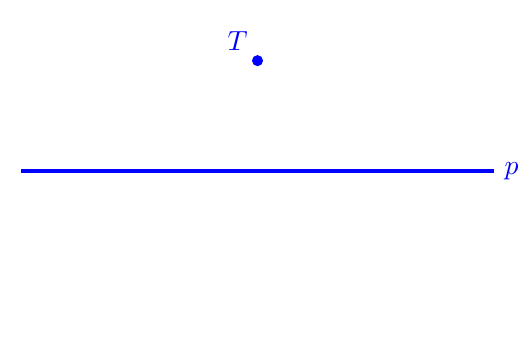
\includegraphics[width=50mm]{fig-1.png}}
            \only<2>{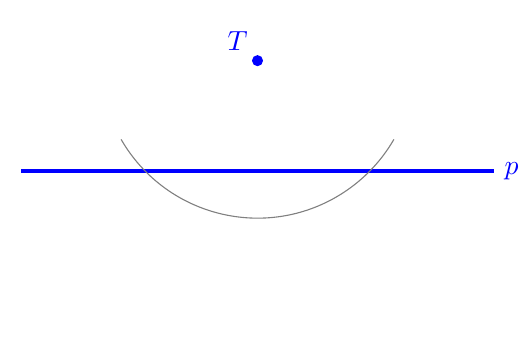
\includegraphics[width=50mm]{fig-2.png}}
            \only<3>{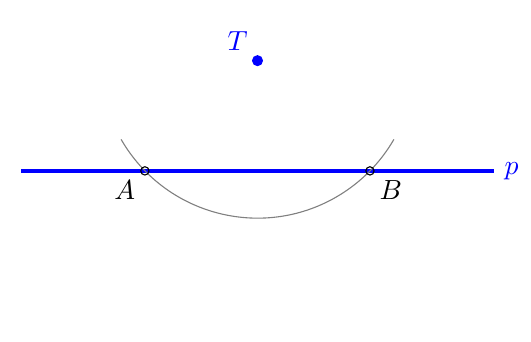
\includegraphics[width=50mm]{fig-3.png}}
            \only<4>{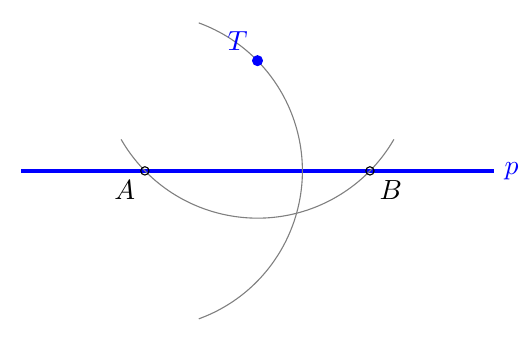
\includegraphics[width=50mm]{fig-4.png}}
            \only<5>{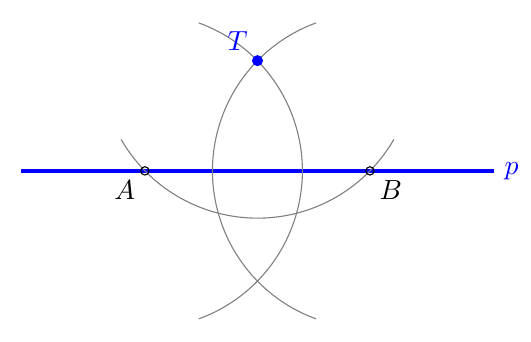
\includegraphics[width=50mm]{fig-5.png}}
            \only<6>{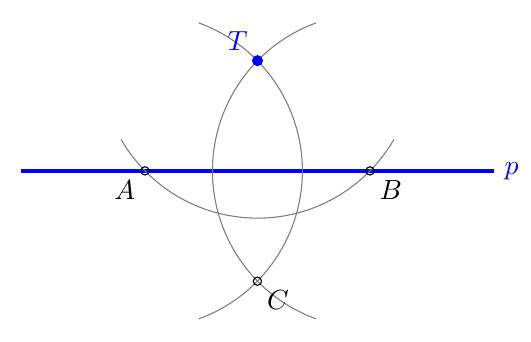
\includegraphics[width=50mm]{fig-6.png}}
            \only<7>{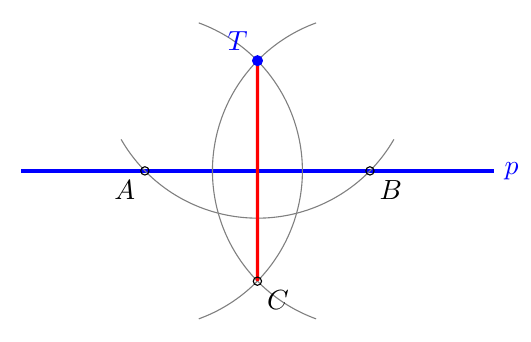
\includegraphics[width=50mm]{fig-7.png}}
        \end{column}
    \end{columns}
\end{frame}
